\documentclass[border=12pt]{standalone}
\def\pgfsysdriver{pgfsys-dvisvgm.def}
\usepackage[dvisvgm]{xcolor}
\usepackage{xeCJK}
\setCJKmainfont{HaranoAjiGothic-Regular.otf}[BoldFont=HaranoAjiGothic-Bold.otf]
\setCJKsansfont{HaranoAjiGothic-Regular.otf}[BoldFont=HaranoAjiGothic-Bold.otf]
\usepackage{amsmath,amssymb,tikz,lmodern}
\usetikzlibrary{arrows.meta,positioning,calc,fit,backgrounds}
\renewcommand{\familydefault}{\sfdefault}
\definecolor{ink}{HTML}{25322F}
\definecolor{green}{HTML}{246657}
\definecolor{tint}{HTML}{EEF4F0}
\definecolor{soft}{HTML}{C6D2CC}
\definecolor{muted}{HTML}{52615B}
\newif\ifJapanese
\newcommand{\Tx}[2]{\ifJapanese #1\else #2\fi}
\newcommand{\Eff}{\overline{\operatorname{Eff}}}
\newcommand{\heading}[3]{{\color{green}\bfseries #1\quad\Tx{#2}{#3}}\\[5pt]}
% A white rectangle makes the complete citation label clickable, including spaces.
\newcommand{\refurl}[2]{\special{dvisvgm:raw <a xlink:href="#1" target="_blank" rel="noopener noreferrer">}{\setlength{\fboxsep}{0pt}\colorbox{white}{\color{green}\underline{\strut #2}}}\special{dvisvgm:raw </a>}}
\tikzset{
 card/.style={draw=soft,fill=white,rounded corners=2pt,align=left,text=ink,font=\fontsize{10.5}{14}\selectfont,inner xsep=12pt,inner ysep=10pt,text width=14.4cm},
 half/.style={card,text width=6.45cm,minimum height=2.05cm},
 result/.style={card,draw=green,fill=tint,line width=.9pt},
 reason/.style={align=left,text=muted,font=\fontsize{9}{12}\selectfont,inner sep=0pt,text width=12.7cm},
 branchreason/.style={reason,text width=5.95cm},
 edge/.style={-{Stealth[length=2.4mm]},draw=green,line width=1pt},
 wire/.style={draw=green,line width=1pt},
}
% Keep the arrow in a dedicated left gutter; explanations never cover it.
\newcommand{\flow}[3]{
 \coordinate (#2-from) at ($(#1.south)+(-6.9,0)$);
 \coordinate (#2-to) at ($(#2.north)+(-6.9,0)$);
 \draw[edge] (#2-from)--(#2-to);
 \node[reason,anchor=west] (#2-reason) at ($(#2-from)!.5!(#2-to)+(.55,0)$) {#3};
}

\newcommand{\Cite}[2]{\refurl{#1}{#2}}

\Japanesefalse
\begin{document}
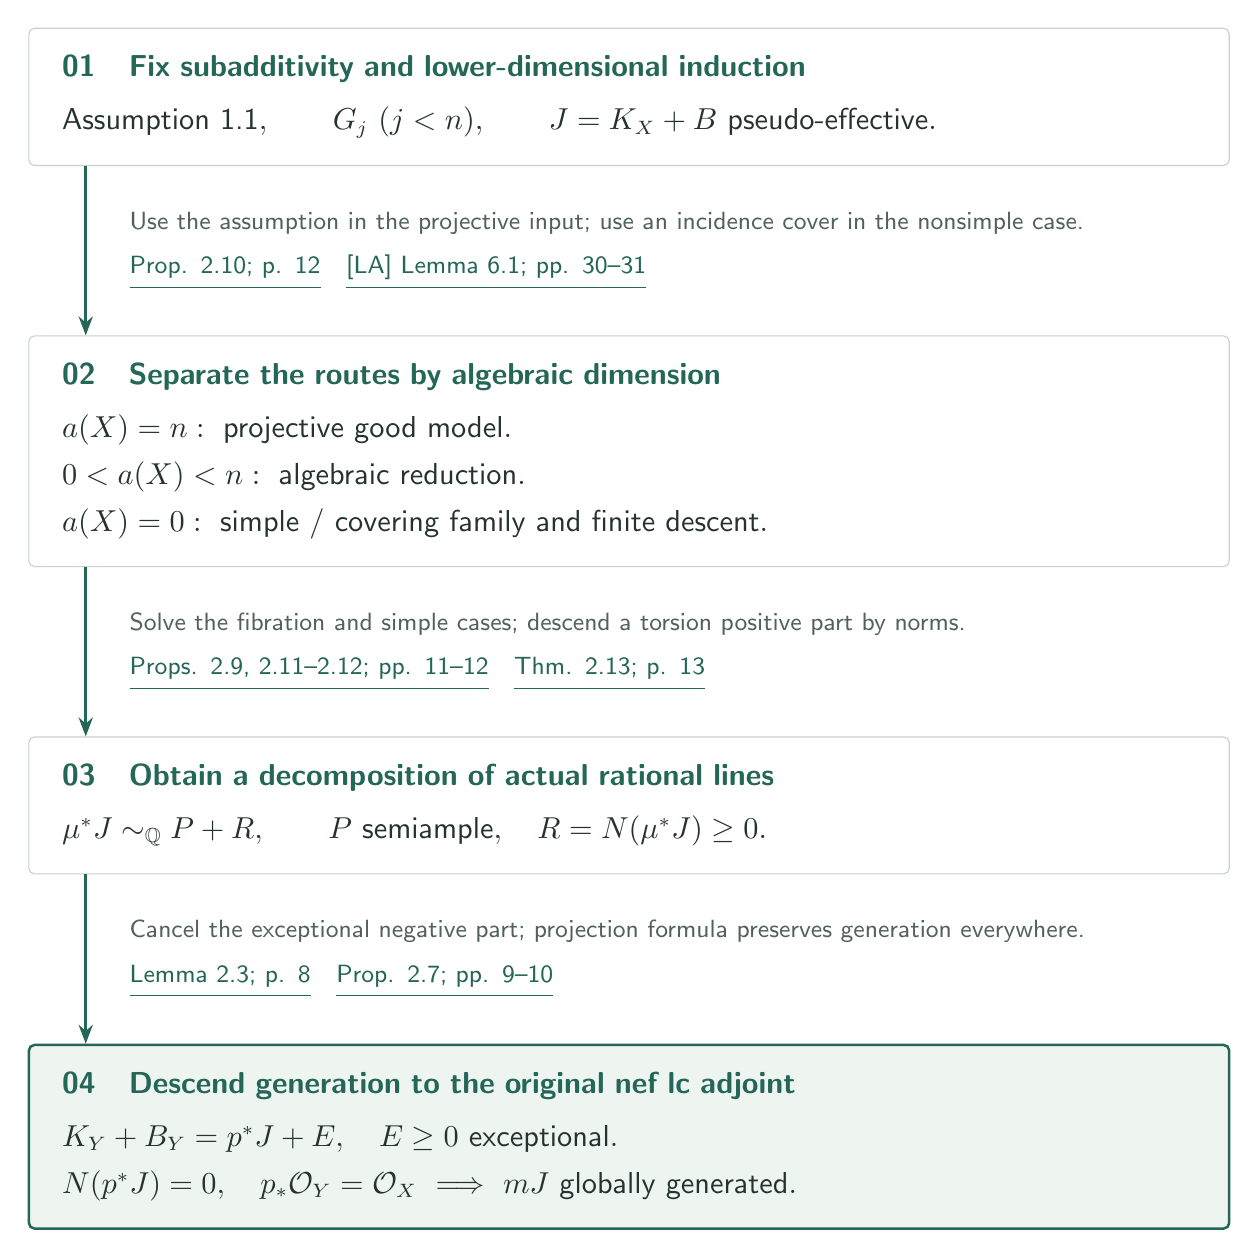
\begin{tikzpicture}
\node[card] (n0) {\heading{01}{劣加法性と下の次元の帰納を固定}{Fix subadditivity and lower-dimensional induction}$\text{Assumption 1.1},\qquad G_j\ (j<n),\qquad J=K_X+B\text{ pseudo-effective}.$};
\node[card,below=2.15cm of n0] (n1) {\heading{02}{代数次元で証明経路を分ける}{Separate the routes by algebraic dimension}$a(X)=n:\ \Tx{\text{射影的good model}}{\text{projective good model}}.$\\[3pt] $0<a(X)<n:\ \Tx{\text{代数的還元}}{\text{algebraic reduction}}.$\\[3pt] $a(X)=0:\ \Tx{\text{simple / 被覆族と有限降下}}{\text{simple / covering family and finite descent}}.$};
\flow{n0}{n1}{\Tx{射影的入力で仮定を使い、非simpleの場合はincidence被覆を作る。}{Use the assumption in the projective input; use an incidence cover in the nonsimple case.}\\[4pt]\Cite{https://github.com/openai/math/blob/adc7f1241b42e322a6451854ab7e4b4c146bf78a/preprints/Log-abundance-for-compact-Kahler-spaces-under-logarithmic-Iitaka-subadditivity-October-4-2026/main.pdf}{Prop. 2.10; p. 12}\quad \Cite{https://github.com/openai/math/blob/adc7f1241b42e322a6451854ab7e4b4c146bf78a/preprints/Log-abundance-in-characteristic-zero-September-24-2026/paper.pdf}{[LA] Lemma 6.1; pp. 30--31}}
\node[card,below=2.15cm of n1] (n2) {\heading{03}{実際の有理直線束の分解を得る}{Obtain a decomposition of actual rational lines}$\mu^*J\sim_{\mathbb Q}P+R,\qquad P\text{ semiample},\quad R=N(\mu^*J)\ge0.$};
\flow{n1}{n2}{\Tx{ファイブレーションとsimpleの場合を解き、torsion正部分をnormで降下。}{Solve the fibration and simple cases; descend a torsion positive part by norms.}\\[4pt]\Cite{https://github.com/openai/math/blob/adc7f1241b42e322a6451854ab7e4b4c146bf78a/preprints/Log-abundance-for-compact-Kahler-spaces-under-logarithmic-Iitaka-subadditivity-October-4-2026/main.pdf}{Props. 2.9, 2.11--2.12; pp. 11--12}\quad \Cite{https://github.com/openai/math/blob/adc7f1241b42e322a6451854ab7e4b4c146bf78a/preprints/Log-abundance-for-compact-Kahler-spaces-under-logarithmic-Iitaka-subadditivity-October-4-2026/main.pdf}{Thm. 2.13; p. 13}}
\node[result,below=2.15cm of n2] (n3) {\heading{04}{元のnefなlc随伴因子へ生成を降下}{Descend generation to the original nef lc adjoint}$K_Y+B_Y=p^*J+E,\quad E\ge0\text{ exceptional}.$\\[3pt] $N(p^*J)=0,\quad p_*\mathcal O_Y=\mathcal O_X\ \Longrightarrow\ mJ\text{ globally generated}.$};
\flow{n2}{n3}{\Tx{例外誤差を負部分から相殺。射影公式で全ての点の生成を保つ。}{Cancel the exceptional negative part; projection formula preserves generation everywhere.}\\[4pt]\Cite{https://github.com/openai/math/blob/adc7f1241b42e322a6451854ab7e4b4c146bf78a/preprints/Log-abundance-for-compact-Kahler-spaces-under-logarithmic-Iitaka-subadditivity-October-4-2026/main.pdf}{Lemma 2.3; p. 8}\quad \Cite{https://github.com/openai/math/blob/adc7f1241b42e322a6451854ab7e4b4c146bf78a/preprints/Log-abundance-for-compact-Kahler-spaces-under-logarithmic-Iitaka-subadditivity-October-4-2026/main.pdf}{Prop. 2.7; pp. 9--10}}
\end{tikzpicture}

\end{document}
